\documentclass[twoside,12pt]{article}

%\usepackage[nodayofweek]{datetime}


\usepackage{multirow}
\usepackage[colorinlistoftodos,disable]{todonotes}
\usepackage[nodayofweek]{datetime}
\usepackage{listings}
\usepackage{graphicx}
\usepackage{titlesec}
\newcommand{\sectionbreak}{\cleardoublepage}
\usepackage[all]{background}
\usepackage{lipsum}
\usepackage{tikz}
\usetikzlibrary{calc}
\usepackage{changepage}
\usepackage{subfigure}
\graphicspath{{Figures/}}

\usepackage{fancyhdr, graphicx}
\renewcommand{\headrulewidth}{0pt}

\fancyfoot[C]{
	\setlength{\unitlength}{1mm}
	\begin{picture}(0,10)
	\put(-70,40){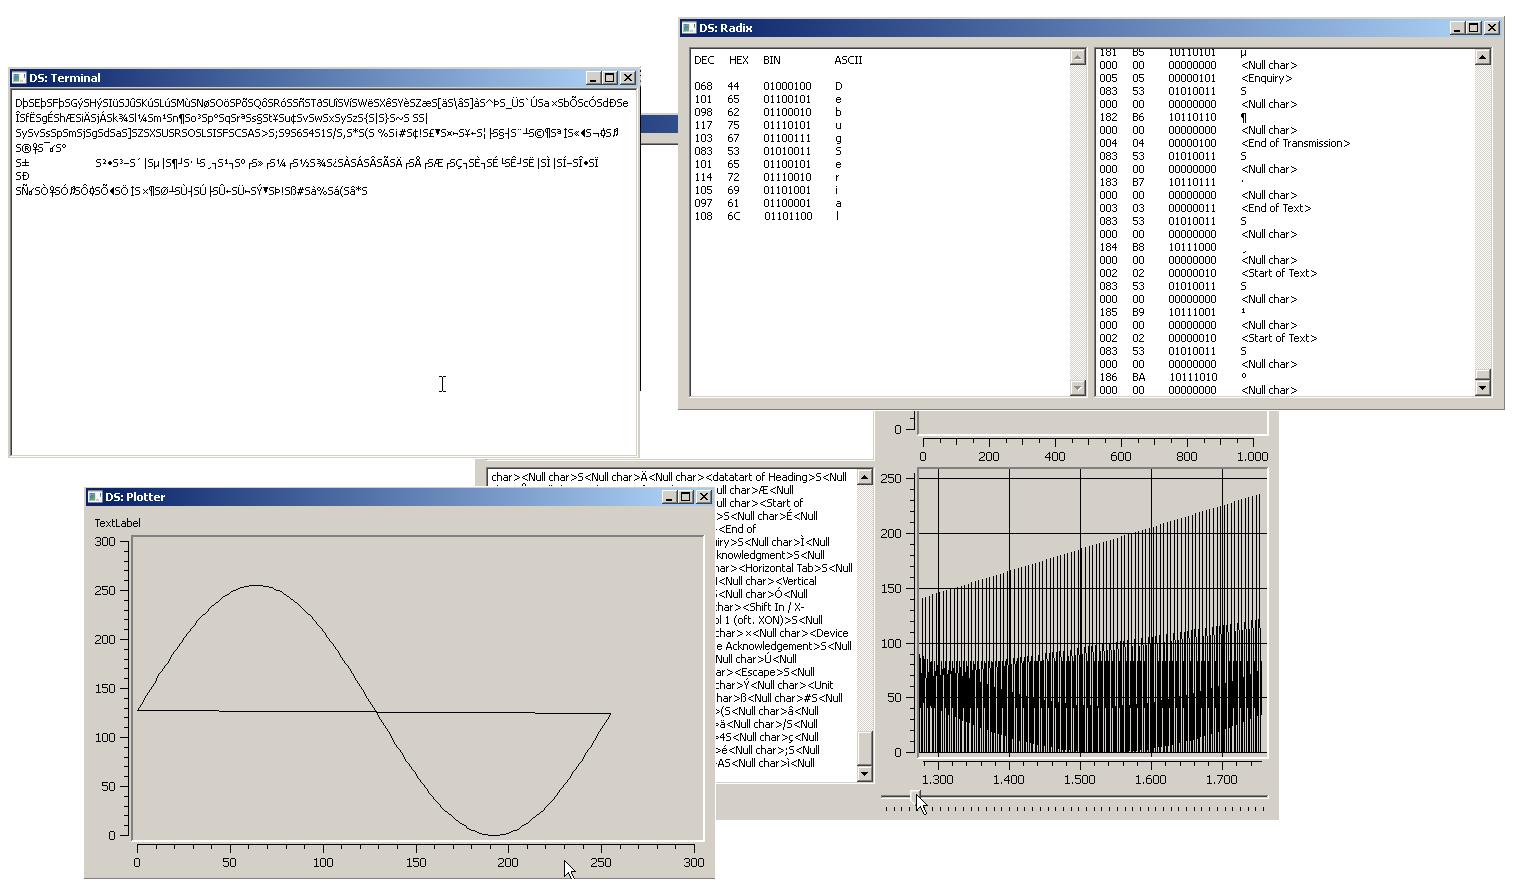
\includegraphics[width=14cm]{cover.jpg}}
	\end{picture}
}


\pagestyle{plain}



\author{
Ashey J. Robinson\\ \texttt{ashley181291@gmail.com}
 \\}

\title{DebugSerial\\ User Manual}

\begin{document}
\maketitle
\thispagestyle{fancy}



\definecolor{mygreen}{rgb}{0,0.6,0}
\definecolor{mygray}{rgb}{0.5,0.5,0.5}
\definecolor{mymauve}{rgb}{0.58,0,0.82}

%Code Styles
\lstset{basicstyle=\scriptsize\ttfamily,
  backgroundcolor=\color{white},   % choose the background color; you must add \usepackage{color} or \usepackage{xcolor}
  basicstyle=\footnotesize,        % the size of the fonts that are used for the code
  breakatwhitespace=false,         % sets if automatic breaks should only happen at whitespace
  breaklines=true,                 % sets automatic line breaking
  captionpos=t,                    % sets the caption-position to bottom
  commentstyle=\color{mygreen},    % comment style
  deletekeywords={...},            % if you want to delete keywords from the given language
  escapeinside={\%*}{*)},          % if you want to add LaTeX within your code
  extendedchars=true,              % lets you use non-ASCII characters; for 8-bits encodings only, does not work with UTF-8
  frame=single,                    % adds a frame around the code
  keepspaces=true,                 % keeps spaces in text, useful for keeping indentation of code (possibly needs columns=flexible)
  numbers=left,                    % where to put the line-numbers; possible values are (none, left, right)
  numbersep=5pt,                   % how far the line-numbers are from the code
  numberstyle=\tiny\color{mygray}, % the style that is used for the line-numbers
  rulecolor=\color{black},         % if not set, the frame-color may be changed on line-breaks within not-black text (e.g. comments (green here))
  showspaces=false,                % show spaces everywhere adding particular underscores; it overrides 'showstringspaces'
  showstringspaces=false,          % underline spaces within strings only
  showtabs=false,                  % show tabs within strings adding particular underscores
  stepnumber=1,                    % the step between two line-numbers. If it's 1, each line will be numbered
  tabsize=2,                       % sets default tabsize to 2 spaces
  title=\lstname                   % show the filename of files included with \lstinputlisting; also try caption instead of title
}


\newcommand*{\FrameXStart}{0.0}% in cm
\newcommand*{\FrameXEnd}{2.0}% in cm
\newcommand*{\FrameYClip}{0.0}% shift in cm of the frame, both from top and bottom
\newcommand*{\FrameTextShift}{-1.5}% shift in cm from the top
\newcommand*{\PageNumberLocation}{4.5}% in cm, from bottom

\newcommand*{\FrameTitle}{DebugSerial: User Manual}%{\ChapterName: \SectionName}%
%
%
%% Style for frame
\tikzset{Frame Style/.style={fill=gray, draw=none, fill opacity=0.5, shade, top color=gray, bottom color=black}}
\tikzset{Title Style/.style={scale=2.75, text=white, rotate=-90, anchor=west}}
\tikzset{Title Top Shift/.style={xshift=\Midpoint cm, yshift=\FrameTextShift cm}}
\tikzset{Title Bottom Shift/.style={xshift=-\Midpoint cm, yshift=\FrameTextShift cm}}

%% Style for page numbers in frame
\tikzset{Page Number Style/.style={scale=2.0, text=white, draw=none}}
\tikzset{Page Number Odd Shift/.style={ xshift= \Midpoint cm, yshift=\PageNumberLocation cm}}
\tikzset{Page Number Even Shift/.style={xshift=-\Midpoint cm, yshift=\PageNumberLocation cm}}
%
\pgfmathsetmacro{\Midpoint}{0.5*(\FrameXStart+\FrameXEnd)}
\newcommand{\MyGraphicLogo}{% For imported graphic logo
\begin{tikzpicture}[remember picture,overlay]
\checkoddpage
\ifoddpage
    \draw [Frame Style] 
        ($(current page.north east)+(-\FrameXStart cm,-\FrameYClip cm)$) rectangle
        ($(current page.south east)+(-\FrameXEnd   cm, \FrameYClip cm)$);
    \node [Title Bottom Shift, Title Style] at (current page.north east) {\FrameTitle};
    \node [Page Number Even Shift, Page Number Style] at (current page.south east) {\thepage};
\else 
    \draw [Frame Style] 
            ($(current page.north west)+(\FrameXStart cm,-\FrameYClip cm)$) rectangle
            ($(current page.south west)+(\FrameXEnd   cm, \FrameYClip cm)$);
    \node [Title Top Shift, Title Style] at (current page.north west) {\FrameTitle};
    \node [Page Number Odd Shift, Page Number Style] at (current page.south west) {\thepage};
\fi 
\end{tikzpicture}
}
%
\SetBgContents{\MyGraphicLogo}% Select frame to be drawn

\SetBgPosition{current page.north west}% Select location
\SetBgOpacity{1.0}% Select opacity
\SetBgAngle{0.0}% Select roation of logo
\SetBgScale{1.0}% Select scale factor of logo
%\pagenumbering{gobble}
\pagestyle{empty}
%import some definitions
\clearpage
%\listoftodos
%\todo[inline]{Run a spell check on all files}
%\begin{abstract}
%Abstract
%\end{abstract}

\newpage
\cleardoublepage
\begin{abstract}

DebugSerial is a tool for debugging embedded software using a simple serial connection.
Only a UART with eight bits of data and a single stop bit is permitted but varying baud rates are allowed.
Motivation for this tool is to increase design potential when only simple hardware is available.
UART protocol is slow but is possible to setup real-time graphs and other interesting analysis techniques.
This software relieves the embedded systems engineer from creating higher level protocols for sending data which can be time consuming when managing both ends of the connections.
Protocols are defined and a rich GUI is provided so debugging using serial is simple from hardware all the way to visualisation.

\end{abstract}
\cleardoublepage
\tableofcontents
\cleardoublepage
\section{Introduction}

\subsection{Hardware}

\subsection{Getting Started}
\ds is invoked as a python script from a terminal window.
\ds will immediately search the environment for all available serial ports.
Failure to find any serial ports will cause \ds to exit.
If only one serial port is available this will be connected to automatically.
When more than one serial port is found a choice will presented.
User choices persist between program executions.

When a serial port is selected a baud rate must be chosen.
Any value can be taken  but this may be limited by chosen hardware.



\end{document}

